\chapter{Undirected Graphical Models}
\label{ch:17}

\begin{exercise}
  A not complete list of conditional independence relations are as follows
  \begin{align}
    & X_1\perp X_3|X_4,\; X_1\perp X_5|X_6,\; X_2\perp X_3|X_4,\; X_2\perp
    X_4|X_1,\; \notag \\
    & X_2\perp X_5|X_6,\;X_3\perp X_5|X_6,\;X_4\perp X_5|X_1
  \end{align}
  The maximal cliques are
  \begin{align}
    \{X_1, X_4\},\;\{X_3, X_4\},\;\{X_5, X_6\},\;\{X_1, X_2, X_6\}
  \end{align}
\end{exercise}

\begin{exercise}
  \begin{exerciseSection}
    \begin{figure}[htb]
      \centering
      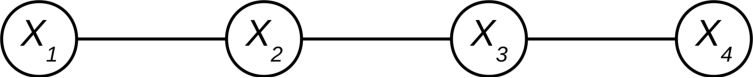
\includegraphics[width=0.4\columnwidth]{./figs/17_2_a.pdf}
      \label{fig:chap_17_2_a}
    \end{figure}
  \end{exerciseSection}
  
  \begin{exerciseSection}
    Same as (a).
  \end{exerciseSection}
  
  \begin{exerciseSection}
    \begin{figure}[htb]
      \centering
      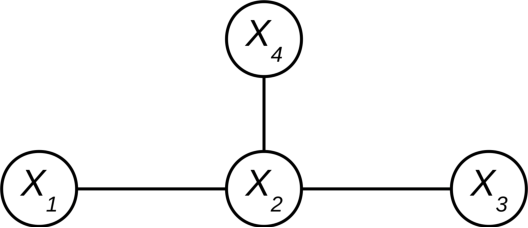
\includegraphics[width=0.3\columnwidth]{./figs/17_2_c.pdf}
      \label{fig:chap_17_2_c}
    \end{figure}
  \end{exerciseSection}
\end{exercise}

\begin{exercise}
  \begin{exerciseSection}
    Since
    \begin{align}
      \left[
        \begin{array}{cc}
          \mathbf{\Theta}_{aa} & \mathbf{\Theta}_{ab} \\
          \mathbf{\Theta}_{ba} & \mathbf{\Theta}_{bb}
        \end{array}
      \right]
      \left[
        \begin{array}{cc}
          \mathbf{\Sigma}_{aa} & \mathbf{\Sigma}_{ab} \\
          \mathbf{\Sigma}_{ba} & \mathbf{\Sigma}_{bb}
        \end{array}
      \right] = \mathbf{I}
    \end{align}
    therefore we have
    \begin{subequations}
      \begin{align}
        \mathbf{\Theta}_{aa}\mathbf{\Sigma}_{aa} +
        \mathbf{\Theta}_{ab}\mathbf{\Sigma}_{ba} = \mathbf{I}
        \label{eq:chap_17_3_a_1}
        \\
        \mathbf{\Theta}_{aa}\mathbf{\Sigma}_{ab} +
        \mathbf{\Theta}_{ab}\mathbf{\Sigma}_{bb} = \mathbf{0}
        \label{eq:chap_17_3_a_2}
      \end{align}
    \end{subequations}
    \eqref{eq:chap_17_3_a_1} -
    \eqref{eq:chap_17_3_a_2}$\mathbf{\Sigma}_{bb}^{-1}\mathbf{\Sigma}_{ba}$, we
    have
    \begin{align}
      \mathbf{\Theta}_{aa}\left(\mathbf{\Sigma}_{aa} -
      \mathbf{\Sigma}_{ab} \mathbf{\Sigma}_{bb}^{-1}\mathbf{\Sigma}_{ba} \right)
      = \mathbf{I}
    \end{align}
    consequently $\mathbf{\Theta}_{aa}^{-1} = \mathbf{\Sigma}_{a, b}$.
  \end{exerciseSection}
  
  \begin{exerciseSection}
    Assume that $\Sigma_{12} = 0$, i.e. $\mathbf{\Sigma}_{aa}$ is diagonal. From
    (a) $\mathbf{\Sigma}_{a, b}$ is also diaonal, which suggests that
    $\mbox{cov}(X_1, X_2|\mbox{rest}) = 0$.
  \end{exerciseSection}
  
  \begin{exerciseSection}
    Since $r_{jk} = \Theta_{jk} / \sqrt{\Theta_{jj} \Theta_{kk}}$, for $j=k$, we
    have $r_{jk} = 1$. For $j\not=k$, denote $X_a = (X_k, X_k)$, then
    \begin{align}
      \left[
        \begin{array}{cc}
          \Theta_{jj} & \Theta_{jk} \\ 
          \Theta_{kj} & \Theta_{kk}
        \end{array}
      \right] = \mathbf{\Theta}_{aa} =
      \left[
        \begin{array}{cc}
          \Sigma_{jj|\mbox{rest}} & \Sigma_{jk|\mbox{rest}} \\ 
          \Sigma_{kj|\mbox{rest}} & \Sigma_{kk|\mbox{rest}}
        \end{array}
      \right]^{-1}
    \end{align}
    therefore
    \begin{subequations}
      \begin{align}
        \Theta_{jj} \Sigma_{jj|\mbox{rest}} + \Theta_{jk}
        \Sigma_{kj|\mbox{rest}} &= 1 \\
        \Theta_{jj} \Sigma_{jk|\mbox{rest}} + \Theta_{jk}
        \Sigma_{kk|\mbox{rest}} &= 0 \\
        \Theta_{kj} \Sigma_{jk|\mbox{rest}} + \Theta_{kk}
        \Sigma_{kk|\mbox{rest}} & = 1
      \end{align}
    \end{subequations}
    consequently, we have
    \begin{subequations}
      \begin{align}
        \Theta_{jj} \Sigma_{jj|\mbox{rest}} & = \Theta_{kk}
        \Sigma_{kk|\mbox{rest}} \\
        \Theta_{jk} \Sigma_{kk|\mbox{rest}} & = \Theta_{jj}
        \Sigma_{jk|\mbox{rest}}
      \end{align}
    \end{subequations}
    As a result, $r_jk = -\Sigma_{jk|\mbox{rest}} /
    \sqrt{\Sigma_{jj|\mbox{rest}} \Sigma_{kk|\mbox{rest}}} =
    -\rho_{jk|\mbox{rest}}$.
  \end{exerciseSection}
\end{exercise}

\begin{exercise}
  Since
  \begin{align}
    f(X_1|X_2, \mbox{rest}) = \frac{f(X_1, X_2| \mbox{rest})}{f(X_2|
    \mbox{rest})} = f(X_1|\mbox{rest})
  \end{align}
  we have
  \begin{align}
    f(X_1, X_2| \mbox{rest}) = f(X_1|\mbox{rest}) f(X_2|\mbox{rest})
  \end{align}
  i.e. $X_1\perp X_2|\mbox{rest}$.
\end{exercise}

\begin{exercise}
  Since there is no missing edges
  \begin{align}
    l_C(\mathbf{\Theta}) = l(\mathbf{\Theta}) = \log|\mathbf{\Theta}| -
    \tr(\mathbf{S\Theta})
  \end{align}
  The gradient equation for maximizing $l_C(\mathbf{\Theta})$ becomes
  $\mathbf{\Theta}^{-1} - \mathbf{S} = 0$, which suggests
  \begin{align}
    \mathbf{S\Theta} = 
    \left[
      \begin{array}{cc}
        \mathbf{S}_{11} & \mathbf{s}_{12} \\
        \mathbf{s}_{12}^T & s_{22}
      \end{array}
    \right]
    \left[
      \begin{array}{cc}
        \mathbf{\Theta}_{11} & \bm{\theta}_{12} \\
         \bm{\theta}_{12}^T & \theta_{22}
      \end{array}
    \right] = 
    \left[
      \begin{array}{cc}
        \mathbf{I} & \mathbf{0} \\
         \mathbf{0}^T & 1
      \end{array}
    \right] 
  \end{align}
  therefore
  \begin{align}
    \mathbf{S}_{11}\bm{\theta}_{12} + \theta_{22}\mathbf{s}_{12} = 0
  \end{align}
  Since $\bm{\beta} = -\bm{\theta}_{12} / \theta_{22}$ as in (17.9), we have
  $\mathbf{S}_{11}\bm{\beta} - \mathbf{s}_{12} = 0$.
\end{exercise}

\begin{exercise}
  Since 
  \begin{align}
    \left[
      \begin{array}{cc}
        \mathbf{W}_{11} & \mathbf{w}_{12} \\
        \mathbf{w}_{12}^T & w_{22}
      \end{array}
    \right]
    \left[
      \begin{array}{cc}
        \mathbf{\Theta}_{11} & \bm{\theta}_{12} \\
         \bm{\theta}_{12}^T & \theta_{22}
      \end{array}
    \right] = 
    \left[
      \begin{array}{cc}
        \mathbf{I} & \mathbf{0} \\
         \mathbf{0}^T & 1
      \end{array}
    \right] 
  \end{align}
  we have
  \begin{subequations}
    \begin{align}
      \mathbf{W}_{11}\bm{\theta}_{12} + \theta_{22}\mathbf{w}_{12} & = 0 \\
      \mathbf{w}_{12}^T\bm{\theta}_{12} + \theta_{22}w_{22} & = 1
    \end{align}
  \end{subequations}
  therefore
  \begin{subequations}
    \begin{align}
      \bm{\theta}_{12} &= -\mathbf{W}_{11}^{-1}\mathbf{w}_{12}\theta_{22} =
      -\hat{\bm{\beta}}\theta_{22} \\
      \theta_{22} &= \frac{1 - \mathbf{w}_{12}^T\bm{\theta}_{12}}{w_{22}}
    \end{align}
  \end{subequations}
  Combining these 2 equations, we have
  \begin{align}
    \theta_{22} = \frac{1}{w_22 -
    \mathbf{w}_{12}^T\mathbf{W}_{11}^{-1}\mathbf{w}_{12}}
  \end{align}
\end{exercise}

\begin{exercise}[(Program)]
\end{exercise}

\begin{exercise}[(Program)]
\end{exercise}

\begin{exercise}
  \begin{exerciseSection}
    \emph{E-step:} The missing data (latent variables), given the current
    estimation $\hat{\bm{\mu}}$, $\hat{\mathbf{\Sigma}}$ and the observed data,
    follow Gaussian distribution as
    \begin{align}
      \mathbf{x}_{i, m_i}\sim\mathcal{N}\left(\hat{\bm{\mu}}_{m_i} +
     \hat{\mathbf{\Sigma}}_{m_i, o_i} \hat{\mathbf{\Sigma}}_{o_i,
      o_i}^{-1} (\mathbf{x}_{i, o_i} - \hat{\bm{\mu}}_{o_i}),
      \hat{\mathbf{\Sigma}}_{m_i, m_i} - \hat{\mathbf{\Sigma}}_{m_i, o_i}
      \hat{\mathbf{\Sigma}}_{o_i, o_i}^{-1} \hat{\mathbf{\Sigma}}_{o_i, m_i}
      \right)
    \end{align}
    (here $\mathbf{x}_{i, m_i}$, $\mathbf{x}_{i, o_i}$ and
    $\hat{\bm{\mu}}_{m_i}$, $\hat{\bm{\mu}}_{o_i})$ are written as column
    vectors.) Therefore, the expectation of the log-likelihood of the data
    over the above conditional distribtion of $\mathbf{x}_{i, m_i}$ is
    \begin{align}
      \mathbb{E}\left[l(\bm{\mu}, \mathbf{\Sigma}; \mathbf{X}_o,
      \mathbf{X}_m)\right] & = C+ N\log|\mathbf{\Sigma}^{-1}| -
      \tr\left(\mathbb{E}\left[(\mathbf{X} - \mathbf{1}\bm{\mu}^T)
      \mathbf{\Theta} (\mathbf{X} - \mathbf{1}\bm{\mu}^T)^T \right] \right)
      \notag
      \\
      &=  C+ N\log|\mathbf{\Sigma}^{-1}|-
      \sum_{i=1}^N
      \sum_{j=1}^p \sum_{k=1}^p\mathbb{E}\left[(x_{ij} - \mu_j)\Theta_{jk}
      (x_{ik} - \mu_k) \right]
    \end{align}
    where $\mathbf{\Theta} = \mathbf{\Sigma}^{-1}$
        
    \emph{M-step: } To maximize the log likelihood, we have
    \begin{align}
      \pdv{\mathbb{E}\left[l(\bm{\mu}, \mathbf{\Sigma}; \mathbf{X}_o,
      \mathbf{X}_m)\right]}{\bm{\mu}} &= \mathbf{1}^T\mathbb{E}[\mathbf{X} -
      \mathbf{1}\bm{\mu}^T]\mathbf{\Theta} = \mathbf{0}
    \end{align}
    thus $\hat{\bm{\mu}} = \mathbb{E}[\mathbf{X}^T\mathbf{1}] / N =
    \hat{\mathbf{X}}^T\mathbf{1} / N$, where $\hat{\mathbf{X}}$ represents the
    $N$-by-$p$ predictor matrix with the missing entries replaced by the imputed
    ones, namely the mean of $\mathbf{x}_{i, m_i}$. Also we have
    \begin{align}
      \pdv{\mathbb{E}\left[l(\bm{\mu}, \mathbf{\Sigma}; \mathbf{X}_o,
      \mathbf{X}_m)\right]}{\mathbf{\Theta}} &= N\mathbf{\Sigma} -
      \mathbb{E} \left[(\mathbf{X} - \mathbf{1}\bm{\mu}^T)^T(\mathbf{X} -
      \mathbf{1}\bm{\mu}^T) \right] = \mathbf{0}
    \end{align}
    therefore, the ML estimation of $\mathbf{\Sigma}$ is
    \begin{align}
      \hat{\mathbf{\Sigma}} = \frac{1}{N} \mathbb{E} \left[(\mathbf{X} -
      \mathbf{1}\hat{\bm{\mu}}^T)^T(\mathbf{X} - \mathbf{1}\hat{\bm{\mu}}^T)
      \right]
    \end{align}
    Denote $E_{ijk} = \mathbb{E}\left[(x_{ij} - \hat{\mu}_j)(x_{ik} -
    \hat{\mu}_k) \right]$, since
    \begin{align}
      E_{ijk} &= (\mathbb{E}[x_{ij}] - \hat{\mu}_j)(\mathbb{E}[x_{ik}] -
      \hat{\mu}_k) + \mbox{cov}(x_{ij}x_{ik})
    \end{align}
    in which 
    \begin{align}
      \mathbb{E}[x_{ij}] = \hat{x}_{ij},\;\mathbb{E}[x_{ik}] = \hat{x}_{ik}
    \end{align}
    whether $j,k\in m_i$ or not, and
    \begin{align}
      \mbox{cov}(x_{ij}x_{ik}) = \left\{
        \begin{array}{ll}
          0 & \mbox{if } j\in o_i \mbox{ or } k\in o_i \\
          \hat{\Sigma}_{jk} & \mbox{otherwise}
        \end{array}
      \right.
    \end{align}
    therefore (17.44) is proved, in which the correction term $c_{i, jj'}$
    corresponds to the the non-zero covariance $\mbox{cov}(x_{ij}x_{ij'})$ when
    both $j$ and $j'$ are imputed for $x_i$.
  \end{exerciseSection}
  
  \begin{exerciseSection}
    (Program)
  \end{exerciseSection}
  
  \begin{exerciseSection}
    (Program)
  \end{exerciseSection}
\end{exercise}

\begin{exercise}
  An absence of the constant node $X_0 \equiv 1$ ill lead to the following
  ambiguity
  \begin{align}
    p(X_1=0, X_2=0) = p(X_1=1, X_2=0) = p(X_1=0, X_2=1)
  \end{align}
  only by including $X_0 \equiv 1$ the 4 possible values can be uniquely
  defined. \begin{figure}[htb]
      \centering
      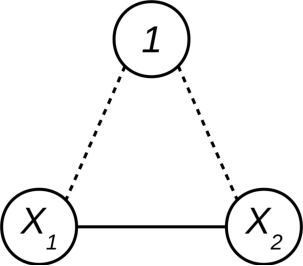
\includegraphics[width=0.15\columnwidth]{./figs/17_10.pdf}
      \label{fig:chap_17_10}
    \end{figure}
\end{exercise}

\begin{exercise}
  \begin{align}
    p(X_j=1|X_{\mbox{rest}} = x_{\mbox{rest}}, \mathbf{\Theta}) &=
    \frac{p(X_j=1,X_{\mbox{rest}} = x_{\mbox{rest}} |
    \mathbf{\Theta})}{p(X_{\mbox{rest}} = x_{\mbox{rest}} | \mathbf{\Theta})}
    \notag \\
    &= \frac{p(X_j=1,X_{\mbox{rest}} = x_{\mbox{rest}} |
    \mathbf{\Theta})} {p(X_j=1, X_{\mbox{rest}} = x_{\mbox{rest}} |
    \mathbf{\Theta}) + p(X_j=0, X_{\mbox{rest}} = x_{\mbox{rest}} |
    \mathbf{\Theta})} \notag \\
    &= \frac{C\exp\left(\sum_{k:(j,k)\in
    E}\theta_{jk}x_k\right)}{C\exp\left(\sum_{k:(j,k)\in E}\theta_{jk}x_k\right)
    + C} \notag \\
    &= \frac{1} 
    {1 + \exp\left(-\sum_{k:(j,k)\in E}\theta_{jk}x_k\right)}
  \end{align}
  where $C$ is a constant given the value of the rest nodes in the graph. Now
  this probability has the logistic form as (17.30) (considering a
  constant node $X_0=1$).
\end{exercise}

\begin{exercise}
  ???
\end{exercise}